\section{Stovepipe Enterprise}

\subsection{Form \& Causes}

Stovepipe Enterprise, also know as Island of Automation \cite{c2com} is a situation when multiple system within enterprise are designed independently at every level \cite{SurvivalGuide}. Those systems has potential to share data, functionality or whole subsystems but they don't.

Stovepipe metaphor isn't accidental. Stovepipe is the pipe which conducts smoke from a coal or wood-burning stove to it's chimney. There are two problems with such pipes and two similar problems will occur in case of stovepipe enterprise anti-pattern. The first problem is that burning wood produces corrosive substances that erode metal, so pipe must be constantly maintained and repaired in order to avoid leakage. Second problem is fact that stovepipes are never connected with each other to create one system. If one would have a two coals he would have two separate stovepipes to maintain.

This analogy perfectly fits into stovepipe enterprise anti-pattern where we have separated systems which has to be maintained separately because of they layer separations. This and other problems will be discussed in the next chapter.

\begin{figure}[!h]
    \centering
    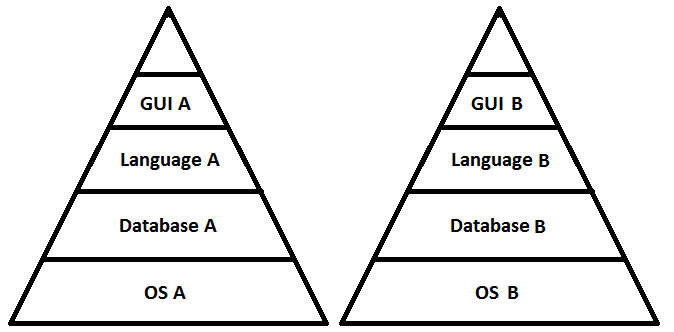
\includegraphics[scale=0.7]{Images/Systems.png}
    \caption[Stovepipe Enterprise Systems]{Stovepipe Enterprise Systems - example visualization}
    \label{fig:Systems}
\end{figure}

Causes of such situations are in general lac of standards, communication and laziness. When a company have global system standards, technology strategy and system profiles then even without teems and enterprise institutions communication such anti-pattern could be avoided. Lack of communication, lack of knowledge about technology standards being used in company and absence of horizontal interfaces in system integration solutions are the main causes of the stovepipe enterprise anti-pattern \cite{SurvivalGuide}.


\subsection{Symptoms \& Consequences}




\subsection{Example - authorization system}

\subsection{Solution}

\subsection{Exceptions}